In this section, flight control is reformulated as a reinforcement learning problem. Afterwards, the IDHP framework is described in terms of both architecture and update rules.

\subsection{RL problem formulation} \label{ssec:rlproblem}
In RL, the interaction between agent and environment is generally modeled as a Markov Decision Process (MDP), and the internal mechanics of the environment are completely hidden from the agent \cite{book:suttonbarto}. In this paper, a modified MDP framework is used where the reward function is a separate entity whose structure is known to the agent. This formulation is often used in ADP literature \cite{Bertsekas2000, Enns2002, Enns2003a, Enns2003b, Ferrari2004,VanKampen2006}.  

Flight control can be described as the process of minimizing the difference between the actual state of an aircraft $s_t$ and a variable reference $s_t^{r}$. Reformulated as an MDP, this can be described as follows. At each timestep t, the agent chooses an action $a_t$ based on the state $s_t$, reference state $s_t^r$, and the current policy $\pi$, as shown in Eq. \eqref{eq:policy}. The environment then provides a scalar reward $r_{t+1}$ and new state $s_{t+1}$. The goal of the agent is to learn a parameterized, deterministic policy, mapping state to action, that maximizes the cumulative sum of future discounted rewards, also known as the return. The mapping of state to expected return is known as the (state-)value function and is described in Eq. \eqref{eq:return_definition}. Here, the parameter $\gamma \in [0,1]$ is called the discount factor.

\begin{equation} \label{eq:policy}
    a_t = \pi( s_t, s_t^R)
\end{equation}
\begin{equation} \label{eq:return_definition}
    V(s_t) = \mathbb{E} \left\{ r_{t+1} + \gamma r_{t+2} + \gamma^2 r_{t+3} + \ldots \right\} = \mathbb{E} \left\{\sum_{k=0}^T \gamma^k r_{t+k+1} \right\}
\end{equation}

In Approximate Dynamic Programming (ADP), the control theory perspective on the reinforcement learning problem, the most common approach is the use of actor-critic methods, also called Adaptive Critic Designs (ACDs). In ACDs, the tasks of action selection and state evaluation are handled by separate structures called Actor and Critic, respectively.

\subsection{Incremental Dual Heuristic Programming} \label{ssec:idhp}

\begin{figure}[h!t]
    \centering
    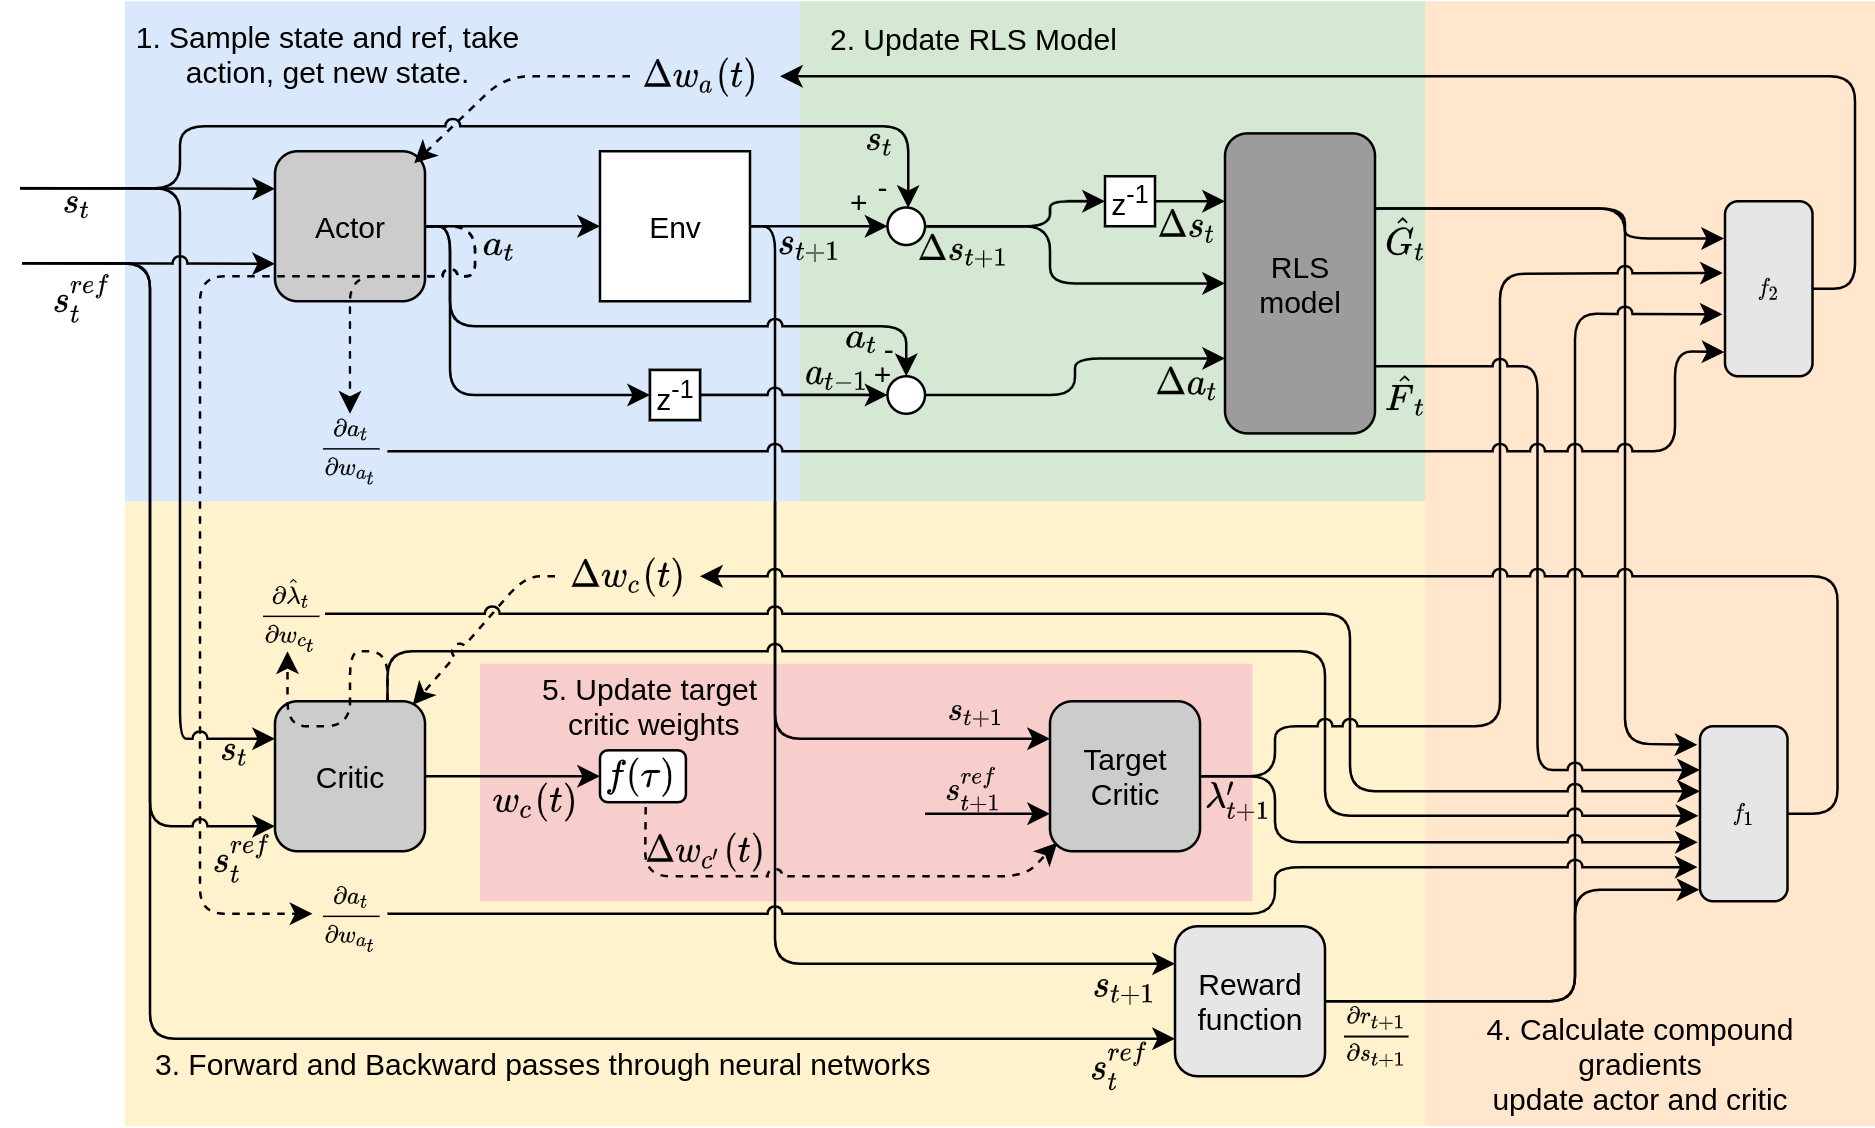
\includegraphics[width=\textwidth]{fig/2/flowchart.png}
    \caption{Flowchart of the information during a single complete time-step of the IDHP learning framework. Solid lines feed-forward information, while dashed lines indicate feed-back update paths. }
    \label{fig:idhp_flowchart}
\end{figure}

The structure of the IDHP agent is based on that first described in \cite{Zhou2018DHP} and expanded upon in \cite{Heyer2020}, and contains four main parametric structures: actor $\pi$, critic $\lambda$, target critic $\lambda'$, and an incremental model of the plant. Fig. \ref{fig:idhp_flowchart} shows how the components of the agent interact with the environment in a single timestep. The colored blocks represent parts of the agent while the white blocks are part of the environment. This section gives an overview of the different parts visible in this model. 

The original IDHP algorithm works forward in time, which requires predicting the states one timestep ahead. This has as an advantage that multiple updates can be done in every timestep, but also means that the accuracy is entirely dependent on the quality of the prediction. In this paper, a backward-in-time approach such as in \cite{Heyer2020, Enns2003a} is chosen. Though this means only a single update can take place every timestep, the high update frequency assumed for the incremental model as described in section \ref{ssec:neuralnetworks} and reduced reliance on forward prediction outweigh this loss.

\subsubsection{Actor and critic neural networks} \label{ssec:neuralnetworks}
In this paper, neural networks are chosen as the function approximator for the actor, critic, and target critic. Specifically, single-hidden-layer fully-connected multi-layered perceptrons (MLPs) are the structure of choice. They are easy to use with RL libraries such as Tensorflow and PyTorch, widely used in RL-for-flight-control literature \cite{Bertsekas2000, Enns2002, Enns2003a, Enns2003b, Ferrari2004, VanKampen2006, Prokhorov1995, Balakrishnan1996, Prokhorov1997, Zhou2016HDP, Zhou2018DHP, Heyer2020}, can theoretically approximate any function arbitrarily well \cite{Hornik1989}, and are differentiable. The critic estimates the partial derivative of the state-value function with respect to the states, while the actor provides a direct mapping between the current state and the action to take. Their structures are shown in Fig. \ref{fig:nn_structure}. The input of both network types is the same: a combination of their respective input states and tracking errors, which are further elaborated on in Section \ref{ssec:controllerdesign}. Both networks use a single hidden layer with ten neurons, using hyperbolic tangent activation functions. The output of the critic and target critic networks consists of a linear output layer with the same dimension as the input. The actor network has a single sigmoid output neuron, corresponding to the required input range of the helicopter model used as explained in Section \ref{ssec:helimodel}.

\begin{figure}[ht]
    \centering
    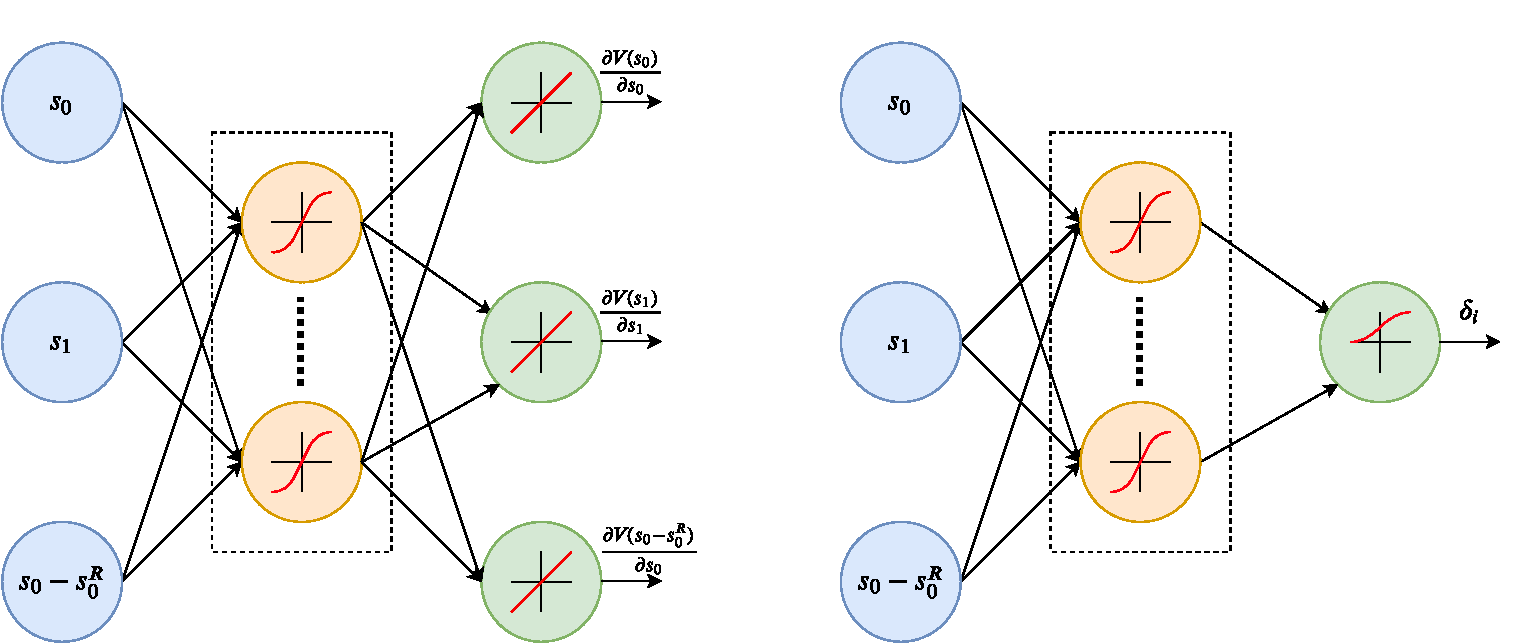
\includegraphics[width=\textwidth, trim={0 0 0.4cm 0.4cm}, clip]{fig/2/NNs2.pdf}
    \caption{Structure of the actor and critic neural networks. Both networks have a single hidden layer with ten neurons. }
    \label{fig:nn_structure}
\end{figure}

\subsubsection{Target critic}
A separate target network as first introduced in \cite{Mnih2015, Lillicrap2015} is often used to stabilize learning in a Deep RL context by decoupling action selection and evaluation. This idea was successfully applied to IDHP in \cite{Heyer2020}, where it was shown that a separate target critic $\lambda'$ with weight vector $w_{c'}$ increased the stability of the learning process at the cost of learning speed. 

\subsubsection{Incremental model} \label{ssec:incrementalrls}
In contrast to older ADP methods, IDHP uses online estimation of an instantaneous linear model identified through Taylor expansion. Consider a discrete-time, nonlinear system $s_{t+1} = f(s_t, a_t)$. A Taylor expansion of this system around $t_0$ yields Eq. \eqref{eq:system_taylor}. By choosing the operating point to be $t_0 = t-1$, a number of new definitions can be made. 
Defining the partial derivatives of the state-transition function to be $F_t = \frac{\partial f(s_t, a_t) }{\partial s_t }$  (the system matrix) and $G_t = \frac{\partial f(s_t, a_t) }{\partial a_t}$ (the control matrix), as well as defining the state and control \textit{increments} to be $\Delta s_t = (s_t - s_{t-1})$ and $\Delta a_t = (a_t - a_{t-1})$, results in the incremental form of the Taylor expansion shown in Eq. \eqref{eq:system_incremental}. Given the assumption of a high sampling rate and slow dynamics, the incremental model form provides a valid linearized, time-varying approximation to the real nonlinear system \cite{Zhou2016iADP}.

\begin{equation}
\label{eq:system_taylor}
    s_{t+1} \approx f(s_{t_0}, a_{t_0}) + \frac{\partial f(s, a) }{\partial s } |_{s_{t_0}, a_{t_0}} (s_t - s_{t_0}) + \frac{\partial f(s, a) }{\partial a } |_{s_{t_0}, a_{t_0}} (a_t - a_{t_0})
\end{equation}
\begin{equation} \label{eq:system_incremental}
    \begin{split}
        s_{t+1} &\approx s_t + F_{t-1} (s_t - s_{t-1}) + G_{t-1} (a_t - a_{t-1}) \\
        \Delta s_{t+1} &= F_{t-1} \Delta s_t + G_{t-1} \Delta a_t
    \end{split}
\end{equation}

\subsubsection{Reward function} \label{ssec:rewardfunction}
In this paper, the reward is designed to be a negative, weighted, squared difference between the reference state and the new actual state, as defined in Eq. \eqref{eq:reward_definition}, with $P \in \mathbb{R}^{p \times n}$ the (Boolean) state selection matrix and $Q \in \mathbb{R}^{p \times p}$ the state weighting matrix. This definition provides the agent with a rich, informative reward signal at each timestep and is inherently differentiable, which is a requirement for the IDHP algorithm explained in section \ref{ssec:idhp}. The derivative of the reward function with respect to the state is given in Eq. \eqref{eq:reward_derivative}.

\begin{equation} \label{eq:reward_definition}
    r_{t+1} = -P\left(s_{t+1} - s_t^r\right)^T QP\left(s_{t+1} - s_t^r\right)
\end{equation}
\begin{equation} \label{eq:reward_derivative}
    \frac{\partial r_{t+1}}{\partial s_{t+1}} = -2P\left(s_{t+1} - s_t^r\right)^TQP
\end{equation}

\subsection{Update rules} \label{ssec:updaterules}
In this section, the update rules for the four parametric structures in the IDHP agent are described in the same order as in which they are updated in each timestep. For brevity, the reference state $s_t^r$, actor weight $w_a(t)$, critic weight $w_c(t)$, and target critic weight $w_{c'}(t)$ are not explicitly shown. Therefore, the four entities in Eq. \eqref{eq:shorthands} are interchangeable.

\begin{equation} \label{eq:shorthands}
    \lambda(s_t, s^R_t, w_c(t)) = \lambda(s_t) \qquad \lambda'(s_t, s^R_t, w_{c'}(t)) = \lambda'(s_t) \qquad \pi(s_t, s_t^R, w_a(t)) = \pi(s_t)
\end{equation}

\subsubsection{Incremental model}
The incremental model is identified through Recursive Least Squares (RLS) estimation. RLS is similar to a Kalman filter, making it very efficient in both computational and memory cost, and avoiding any potential problems with matrix inversions. The current state and control matrix are estimated together in one parameter matrix $\hat{\Theta}_t$, as shown in Eq. \eqref{eq:rls1}. 
\begin{equation} \label{eq:rls1}
    \hat{\Theta}_{t-1} = \begin{bmatrix} \hat{F}^T_{t-1} \\ \hat{G}^T_{t-1}\end{bmatrix}
\end{equation}
The parameter matrix is accompanied by a covariance matrix $P_t$, which provides an indication of the reliability of the parameter estimates. For the update process, first, a prediction of the next state increment, $\Delta \hat{s}_{t+1}$, is made using the current state and action increments as well as the current parameter matrix, as shown in Eqs. \eqref{eq:rls2} and \eqref{eq:rls3}. 
\begin{equation} \label{eq:rls2}
    X_t = \begin{bmatrix} \Delta s_t \\ \Delta a_t \end{bmatrix}
\end{equation}
\begin{equation} \label{eq:rls3}
    \Delta \hat{s}_{t+1} = \left(X_t^T \hat{\Theta}_{t-1}\right)^T
\end{equation}
This prediction is then compared with the actual state increment, and the prediction error, also known as innovation, is computed as $\epsilon_t = (\Delta s_{t+1} - \Delta \hat{s}_{t+1})^T$. Finally, the parameter and covariance matrices are updated according to Eqs. \eqref{eq:rls4} and \eqref{eq:rls5}, respectively, where $\kappa \in [0,1]$ is the scalar forgetting factor, which exponentially decays the importance of older measurements. 
\begin{equation} \label{eq:rls4}
    \hat{\Theta}_{t} = \hat{\Theta}_{t-1} + \frac{\hat{P}_{t-1} X_t \epsilon_t}{\kappa + X_t^T \hat{P}_{t-1} X_t}
\end{equation} 
\begin{equation} \label{eq:rls5}
    \hat{P}_t = \frac{1}{\kappa}\left[\hat{P}_{t-1} - \frac{\hat{P}_{t-1} X_t X_t^T \hat{P}_{t-1}}{\kappa + X_t^T \hat{P}_{t-1} X_t}\right]
\end{equation}

\subsubsection{Critic}
The critic in IDHP estimates the partial derivative of the state-value function with respect to the states: $\lambda(s_t, s^R_t) = \frac{\partial V(s_t, s^R_t)}{\partial s_t}$. The critic is updated by means of a one-step temporal difference (TD) backup operation that minimizes the mean-squared error of the critic error: $L_C = \frac{1}{2}e_c^2$. The critic error is the partial derivative of the one-step TD error with respect to the state vector as defined in Eq. \eqref{eq:critic_error}. 

\begin{equation} \label{eq:critic_error}
    \begin{split}
        e_c &= -\frac{\partial \left[ r(s_{t+1}, s^R_t) + \gamma V(s_{t+1}) - V(s_t) \right]}{ \partial s_t} \\
        &= -\left[\frac{\partial r(s_{t+1}, s^R_t)}{ \partial s_{t+1}} + \gamma \lambda'(s_{t+1}, s^R_{t+1})\right] \frac{\partial s_{t+1}}{\partial s_t } + \lambda(s_{t}, s^R_t)
    \end{split}
\end{equation}

The value of the next state $s_{t+1}$ is dependent on both the previous state and the action. Therefore, its derivative with respect to the previous state, which is the final term in Eq. \eqref{eq:critic_error}, must be expanded to contain both these pathways. The approximations to the new derivative terms, obtained previously from the RLS model, as well as the backpropagation result of the state through the actor network, can then be substituted to yield Eq. \eqref{eq:dst+1_ds}. 
\begin{equation} \label{eq:dst+1_ds}
\begin{split}
    \frac{\partial s_{t+1}}{\partial s_t } &= \frac{\partial f(s_t, a_t)}{\partial s_t } + \frac{\partial f(s_t, a_t)}{\partial a_t } \frac{\partial a_t}{\partial s_t} \\
    &= \hat{F}_{t-1} + \hat{G}_{t-1} \frac{\partial \pi(s_t, s^R_t, w_c)}{\partial s_t}
\end{split}
\end{equation}
Finally, the critic weights are updated through gradient descent on the critic loss, with learning rate $\eta_c$, as shown in Eqs. \eqref{eq:critic_update} and \eqref{eq:critic_update_2}.
\begin{equation} \label{eq:critic_update}
    w_c(t+1) = w_c(t) + \Delta w_c(t)
\end{equation}
\begin{equation} \label{eq:critic_update_2}
\begin{split}
    \Delta w_c(t) &= -\eta_c \frac{\partial L_C}{\partial w_c } =  -\eta_c \frac{\partial L_C}{\partial \lambda(s_{t}, s^R_t, w_c(t))} \frac{\partial \lambda(s_{t}, s^R_t, w_c(t))}{\partial w_c(t)} \\
    &= -\eta_c e_c(t) \frac{\partial \lambda(s_{t}, s^R_t, w_c(t))}{\partial w_c(t)}
\end{split}
\end{equation}

\subsubsection{Actor}
The goal of the actor is to find a policy which maximizes the state-value function: the optimal policy $\pi^*$. Consequently, the optimal action $a^*$ is defined as:
\begin{equation} \label{eq:optimalpolicy}
    a^*_t = \pi^*(s_t, s^R_t, w_a(t)) = arg \max_{a_t} V(s_t, s^R_t)
\end{equation}
Because the update takes place after a state transition, the TD(0) expansion of this value can be maximized instead. Consequently, the loss function to minimize with gradient descent is the negative TD(0) target, as shown in Eq. \eqref{eq:actorloss}.
\begin{equation} \label{eq:actorloss}
    L_A = -V(s_t, s^R_t) = -\left[ r(s_{t+1}, s^R_t) + \gamma V(s_{t+1}, s^R_{t+1}) \right]
\end{equation}
The state-value function is not directly dependent on the weights of the actor. Therefore, the update path takes place through the critic, reward function and environment model instead, as shown in Eq. \eqref{eq:actorlossderiv}.
\begin{equation} \label{eq:actorlossderiv}
\begin{split}
    \frac{\partial L_A}{\partial w_a} &= -\frac{\partial \left[ r(s_{t+1}, s^R_t) + \gamma V(s_{t+1}, s^R_{t+1}) \right]}{\partial a_t}\frac{\partial a_t}{\partial w_a } \\
    &= -\left[ \frac{\partial r_t}{\partial s_{t+1} } + \gamma \frac{\partial V(s_{t+1})}{\partial s_{t+1} } \right] \frac{\partial s_{t+1}}{\partial a_t } \frac{\partial a_t}{\partial w_a } \\
    &= -\left[ \frac{\partial r_t}{\partial s_{t+1} } + \gamma \lambda'(s_{t+1}) \right] G_{t-1} \frac{\partial \pi(s_t)}{\partial w_a }
\end{split}
\end{equation}

As with the critic, the actor weights are updated through gradient descent with learning rate $\eta_a$, as shown in Eq. \eqref{eq:actorupdate}.

\begin{equation} \label{eq:actorupdate}
    w_a(t+1) = w_a(t) + \Delta w_a(t) = w_a(t) - \eta_a \frac{\partial L_A}{\partial w_a}
\end{equation}

\subsubsection{Target critic}
Finally, the target critic is updated towards the critic using soft updates \cite{Lillicrap2015}, also known as Polyak averaging \cite{Lee2019}, as shown in Eq. \eqref{eq:targetcriticupdate}, where $\tau$ indicates the (usually small) mixing factor. 

\begin{equation} \label{eq:targetcriticupdate}
    w_{c'}(t+1) = \tau w_{c}(t+1) + (1-\tau) w_{c'}(t)
\end{equation}

% \frac{\partial }{\partial  }